Dans ce chapitre (section \ref{sConGameConcept}), la conception du SG est décrite telle qu'il devrait être d'après la description du projet R\&D. Cette conception cherche à répondre à tous les objectifs identifiés précédemment dans l'Analyse (section \ref{sAnaDescriptionObjectifsCTI}) et à être compatible avec le plus de points importants mis en avant (section \ref{sAnaGameConceptPointsImportant}). L'ensemble de ces objectifs et donc du SG conçu n'est pas implémenté dans ce travail, une sélection est faîte et détaillée dans la section \ref{sConSelectionObjectifs}. Les principaux risques concernant l'implémentation de cette sélection d'objectifs sont ensuite décrits dans la section \ref{sConIdentificationRisques}. Les approches permettant de minimiser leurs probabilité d'apparition ainsi que leurs impacts y sont décrites également. Ce chapitre se conclut par une description de la communication conçue (section \ref{sConCommunication}).

\section {Concept du jeu}
	\label{sConGameConcept}
	Le concept global du jeu est l'exploration de planètes à la recherche de traces d'une civilisation disparue. Ce concept permet de correspondre aux objectifs du projet R\&D (section \ref{sAnaDescriptionObjectifsCTI}) mais également aux points importants à prendre en compte lors de la conception d'un tel SG (section \ref{sAnaGameConceptPointsImportant}). Il a été élaboré avec le Prof. Dr. Stéphane Gobron (professeur d'infographie, responsable de l'ancien projet SG4R et du projet à venir) de la HES-SO Neuchâtel et le Prof. Dr. Michel Lauria (responsable des équations de mouvements du projet SG4R et du projet à venir) de la HES-SO Genève. Ce concept a ensuite été validé par le mandant. Celui-ci ainsi que ses possibilités sont présentés en détails dans les sous-sections à venir.
	
	\subsection*{Histoire du jeu}	
		Après de nombreuses années de voyage, le vaisseau d'exploration arrive dans une galaxie avec de nombreuses planètes qui offraient ou semble offrir les conditions idéales pour le développement d'une civilisation. C'est au joueur d'explorer ces planètes afin de trouver des traces de cette civilisation. Le but étant de découvrir ce qu'elle est devenue.
		Le voyage spatial ayant duré de nombreuses années, les membres de l'équipage ont les muscles atrophiés et sont obligés d'explorer les planètes en commençant par celles ayant peu de gravité.
	
	\subsection*{Élémentss différentiateur}		
		Comparé aux autres SGs développés pour le LHS, celui-ci propose un scénario et une grande possibilité d'amélioration. De plus, les paramètres thérapeutiques tels que l'assistance, la gravité ou l'appauvrissement de la scène ont un sens dans le scénario (\textit{e.g.}, constante de gravité de la planète pour l'assistance du robot). De plus, ce SG peut poser une base pour de futurs, ou dores et déjà existant, SG pouvant être liés tout en proposant d'autres exercices et ainsi, à long terme, rejoindre l'idée de plateforme (utilisation de véhicule pour du pédalage ou encore session de vol pour rejoindre le vaisseau, ce qui peut correspondre au SG \textit{SpaceGate}).
	
	\subsection*{Environnement virtuel}
		L'environnement est composé de l'intérieur du vaisseau spatial ainsi que la surface des différentes planètes à explorer.
		
		L'intérieur du vaisseau spatial est une zone contenant des objets familiers (table, chaise, cadre, etc.). Elle sert également de zone de transfert entre la salle où se trouve le patient et une réalité virtuelle sur une planète inconnue. Cette zone doit être neutre et pouvoir ressembler à une salle d'hôpital. Le patient devra la traverser en marchant afin d'en sortir, offrant ainsi une transition entre les deux types d'environnement et inversement. Le joueur s'y trouve donc au début et à la fin de chaque session de jeu.
		
		Les planètes peuvent, elles, être très différentes. Composées de terrains désertiques contenant seulement des rochers, peu de couleurs (mars) et aucun voire peu de sons, comme celle maquettée en figure \ref{Maquette}. À l'inverse, ce peut être une planète contenant beaucoup d'êtres vivants tels que des arbres et des animaux, très riche en couleurs, formes et sons. L'appauvrissement ou l'enrichissement de tels mondes inconnus peut être plus cohérent que s'il s'agissait d'endroit connus. 
		
		Le SG contient différents types de sols avec différentes textures, effets sonores et sensations haptiques. Il peut également contenir des pentes et marches. La présence de points d'eau (changeant le coefficient de viscosité) peut permettre une immersion progressive.\medskip			
		
		%TODO: Uniformiser couleurs, tailles et polices des légendes
		\begin{minipage}{\linewidth}
			\makebox[\linewidth]{
				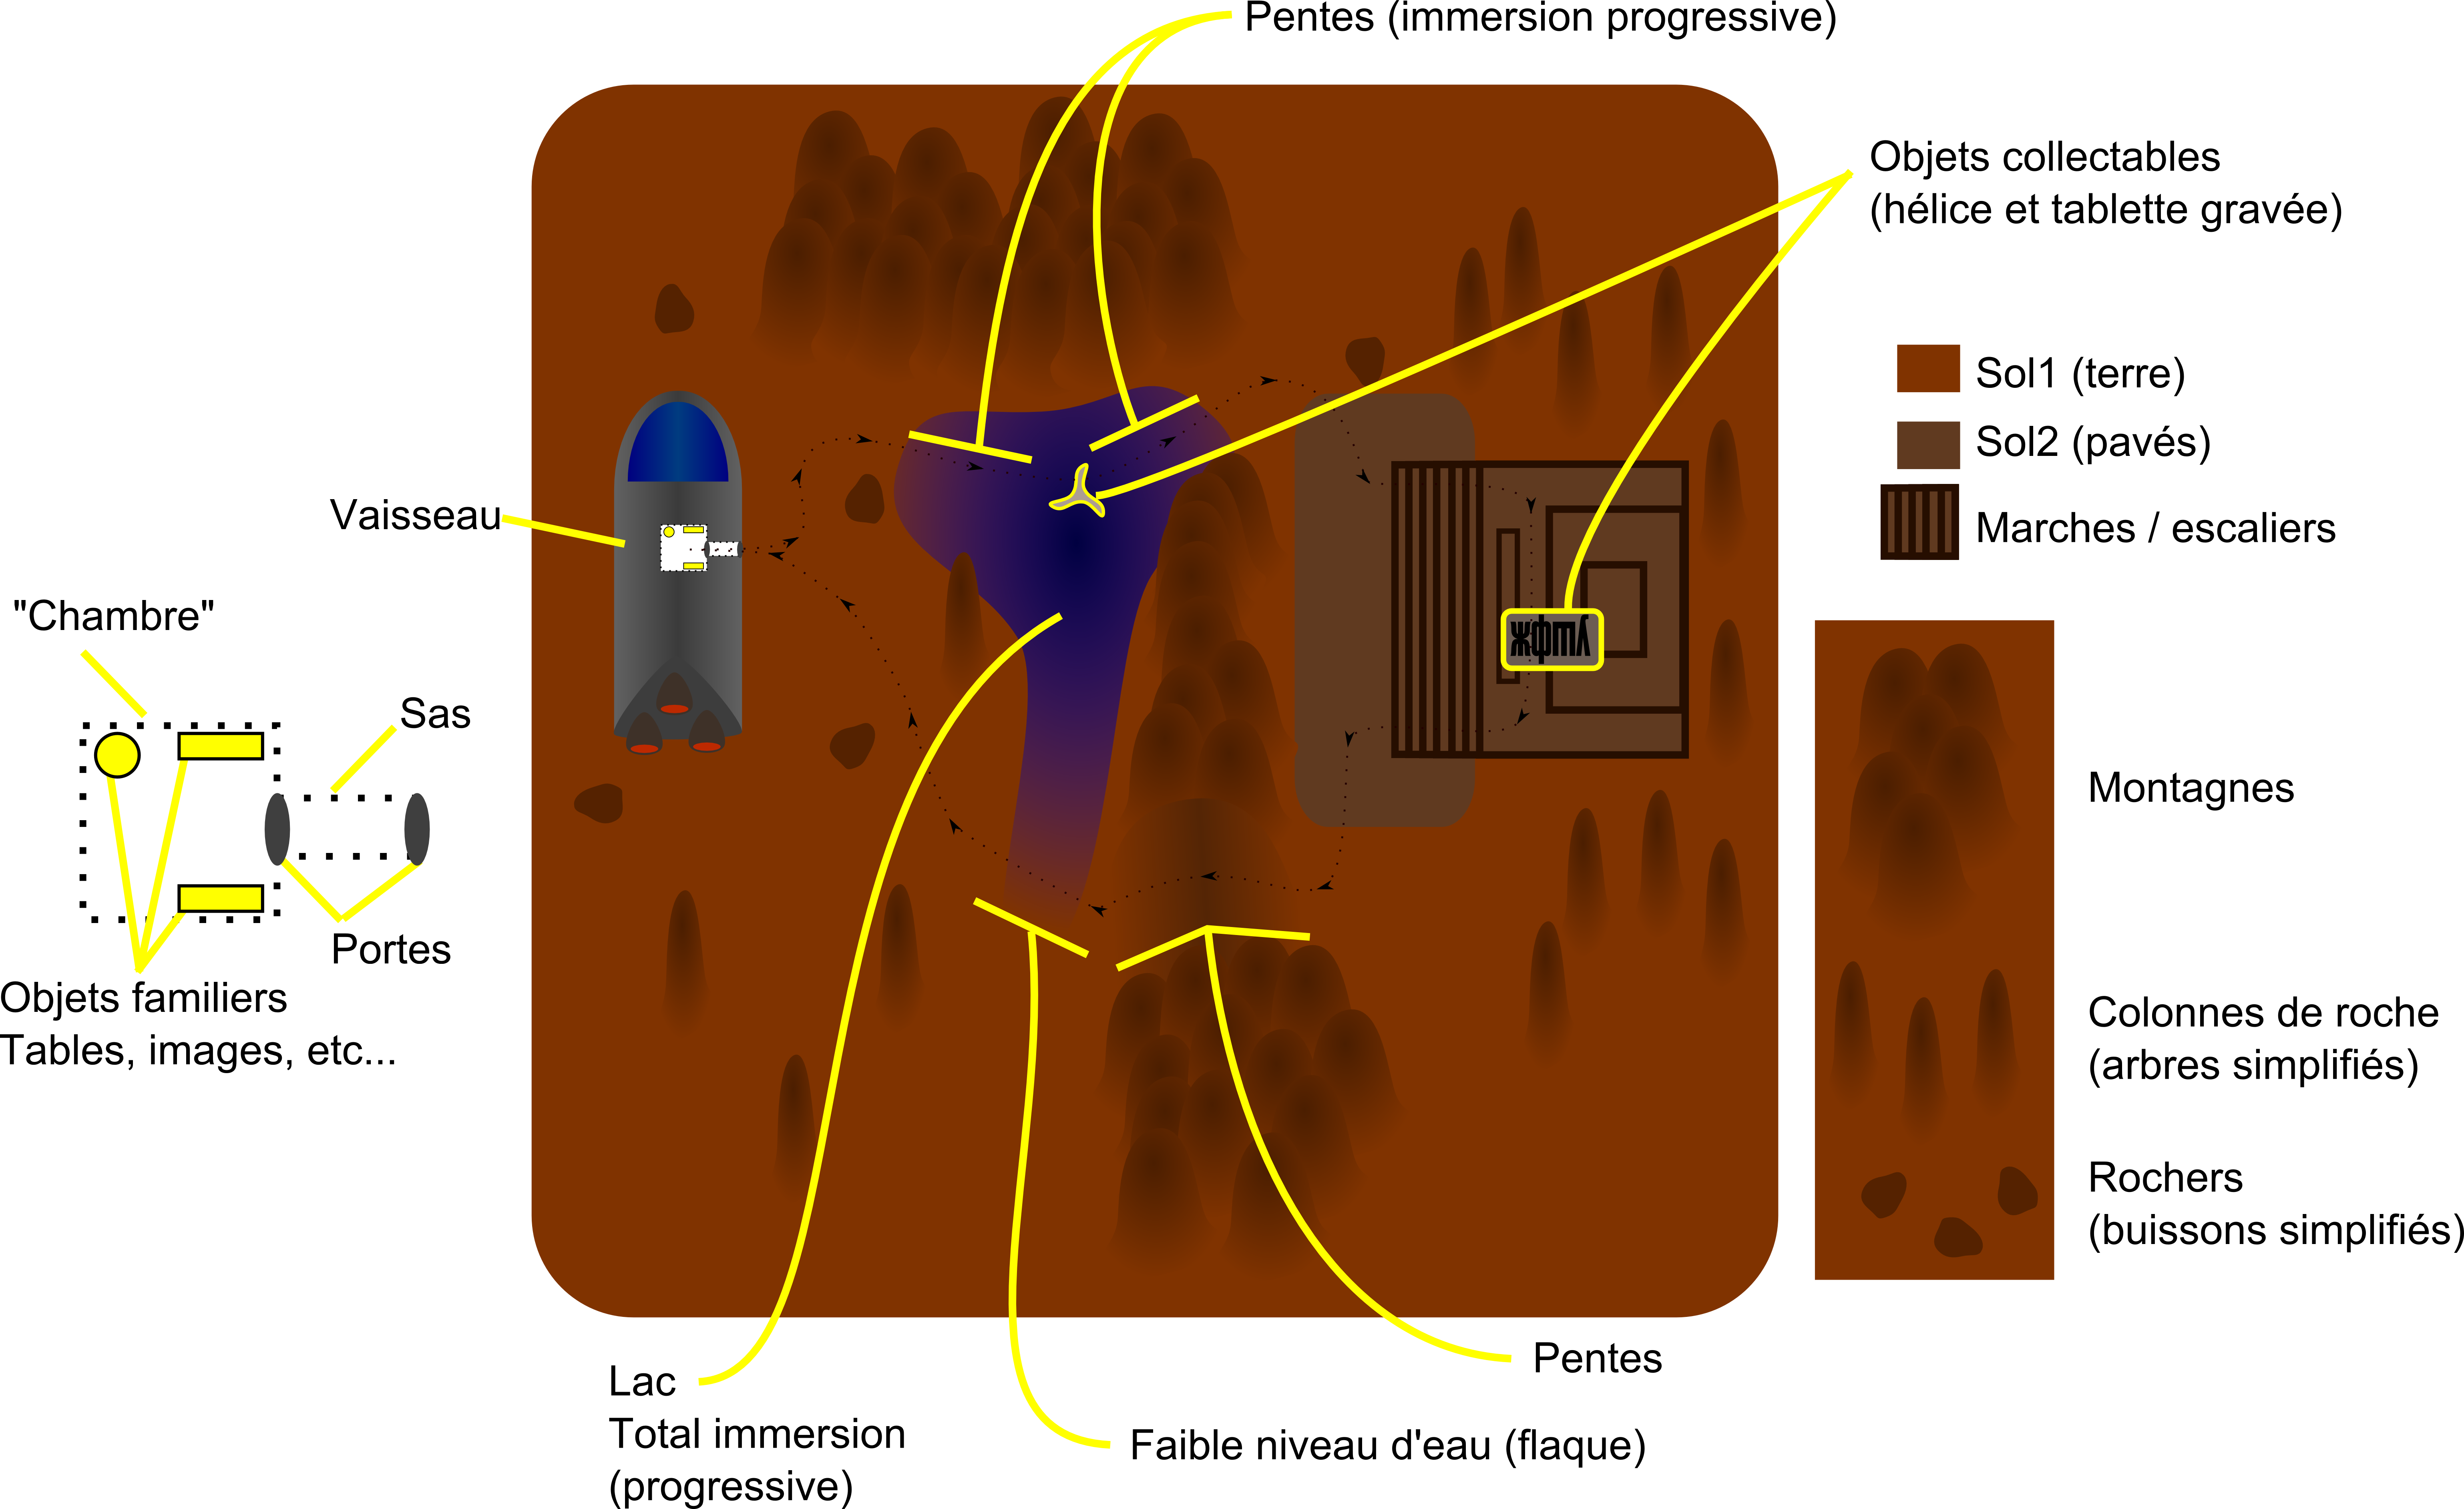
\includegraphics[width=\textwidth]{img/Conception_MaquetteAvecLegende.png}}
			\captionof{figure}{Maquette de l'environnement du jeu avec le parcours et les éléments à trouver.}
			\label{Maquette}
		\end{minipage}\medskip		
		
	\subsection*{Gameplay}
		Une session de jeu effectue un niveau qui consiste en une "sortie" sur une planète. Celle-ci suit un parcours bien défini que le joueur ne peut modifier. Le but étant de trouver et collecter des indices sur cette civilisation. Les mécanismes de recherche et de collecte pourront évoluer au cours de la réhabilitation (cf. sous-section suivante). Les deux principaux arguments ayant menés à la décision d'un chemin défini sont les suivants: simplicité d'interaction et simplicité des modèles mathématiques. Un déplacement libre aurait implicitement dû ajouter un moyen de tourner et, par conséquent, une interaction supplémentaire, ce qui n'est pas souhaitable. L'hypothèse d'effectuer la rotation par rapport au regard est exclue car ce n'est pas une façon naturelle de se déplacer (et aurait donc put nuire à la neuroréhabilitation) et cela interfère avec toutes autres interactions de recherche dans l'environnement (primordiale pour trouver les traces de la civilisation). L'autre raison (simplicité des modèles mathématiques) provient des contraintes pour la modélisation mathématique du mouvement en tenant compte du type de sol. La complexité est nettement diminuée si, dès l'initialisation du SG, les modèles peuvent connaître toutes les pentes et types de sols du parcours. Dans le cas contraire, même durant le projet R\&D, ce modèle ne pourrait être implémenté.
		\\
		
		Le challenge du jeu est alors de collecter suffisamment d'indices lors d'une sortie pour pouvoir passer au point d'exploration suivant (ailleurs sur la planète ou sur une autre). Le nombre d'indices peut être indiqué à l'avance (\textit{e.g.}, "Six artéfacts correspondant à la signature fréquentielle de la civilisation ont étés détectés"). Des indicateurs peuvent être mis en place si le joueur effectue plusieurs fois la même sortie sans trouver d'indices (\textit{e.g.}, "Des scans approfondis ont permis de localiser plus précisément les artéfacts"). Si ce challenge est jugé insuffisant, un score ou une appréciation peuvent être réalisés par la suite en fonction du nombre d'objectifs trouvés, l'aide nécessaire, l'énergie dépensée, l'état de la combinaison spatiale, etc. Bien que certains de ces éléments soient dépendants d'interactions spécifiques n'intervenant pas en début de thérapie.	
		\\
		
		On peut également imaginer une progression faisant corréler l'avancement du SG avec une réhabilitation cognitive. Le patient commencerait par des planètes "désertiques" et, au fur et à mesure de sa réhabilitation, découvrirait des planètes plus riches (abandonnées depuis moins longtemps). Ce schéma de progression est cependant grandement lié au profil des patients (certains n'auront aucun troubles cognitifs alors que d'autres pourront peut-être réapprendre à marcher mais uniquement dans des endroits appauvris). Afin de ne pas se restreindre à un profil précis et de permettre la progression du SG et de la réhabilitation motrice à la plus grande plage de patients, aucune progression de ce style ne doit être présente. Il pourrait cependant être intéressant de voir s'il est possible d'établir des profils de patients et ainsi de proposer une progression en relation.
		
	\subsection*{Personnages et contrôles}
		Le joueur contrôle un avatar à la première personne. Toutes les parties se font avec un autre personnage non joueur que l'on devra suivre. Celui-ci effectue un mouvement de marche correcte et sert à l'activation des neurones miroirs mais peut également être la représentation du thérapeute, lui donnant des conseils dans sa réhabilitation. La principale interaction étant donc la marche via le LHS pour faire avancer l'avatar, les rotations devant être légères et automatiques (parcours défini et non libre). Des obstacles à éviter (flaque / cailloux) pourront être utilisés pour rendre le patient plus conscient de ses mouvements si cela est souhaitable par les thérapeutes. Cela ne rentre cependant pas dans le cadre du premier produit à réaliser. Les sorties auront un temps défini (durée de l'exercice) lié à l'oxygène de la combinaison spatiale. En conséquent, les pauses durant l'exercice doivent être évitées.
		
		La façon dont les indices sont recherchés et collectés peut évoluer au long de la réhabilitation pour correspondre au besoin d'ajout d'interactions (voir analyse, section \ref{sAnaGameConceptPointsImportant}). Par exemple, au début, l'autre personnage peut réussir à découvrir quelques indices, le joueur doit juste le suivre. Par la suite, le joueur peut indiquer les objets à collecter en les fixant du regard (HMD). Ensuite il pourrait les collecter ou prendre des photos d'éléments intéressants via contrôle vocal/simple bouton. Finalement, d'autres interactions peuvent être mises en place telles qu'un zoom, une détection radar, etc.
		
	\subsection*{Choix techniques}
		Pour les raisons détaillées dans l'analyse (section \ref{sAnaContraintes}), le SG sera développé avec \textit{Unity} avec des scripts en \textit{C\#}. Les modèles 3D devront être trouvés sur internet. %TODO: Dire que c'est pas justifier/raisonnable de passet 1j à la création d'un truc alors qu'un designer le fait en une heure ?
		L'avatar (ses jambes) devra être animé d'après les angles et positions des segments corporels calculés par le LHS. Les différentes modalités de retour devront être garanties à une fréquence où aucun délai n'est perceptible par l'utilisateur (détaillé dans l'analyse, section \ref{sAnaGameConceptPointsImportant}).
		Le SG tournera sur un PC dédié et communiquera avec le noyau temps réel ainsi que de l'IHM. Le PC ne contiendra qu'un écran, un \textit{Oculus Rift} et d'éventuels autres périphériques pour le SG (micro, bouton, manette de jeux, etc.). Il devra se lancer automatiquement et contenir un minimum de paramètres ou interfaces accessibles au patient pour démarrer la partie au plus vite.
		

\section{Sélection des objectifs}
\label{sConSelectionObjectifs}
	Dans cette section sont repris tous les objectifs du projet R\&D décrits dans l'analyse, section \ref{sAnaDescriptionObjectifsCTI}. Ils sont triés par ordre de priorité décroissant. Chaque sous-section décrit ce que le SG à développer durant ce travail doit contenir et ce qui est laissé au projet suivant (le SG devant faciliter leur future intégration).
	\subsection*{Niveaux d'appauvrissement}
		Pour les niveaux d'appauvrissement, il est décidé de pouvoir travailler sur différents aspects: densité des objets; modélisation géométrique; audio; rendu des couleurs; animations; effets de lumière. Le SG fournit donc plusieurs variables pouvant être modifiées à souhait et offre ainsi de nombreuses combinaisons possibles. Par la suite, pour simplifier la configuration, le thérapeute n'aurait accès qu'à une variable "Appauvrissement" et chaque aspect serait définit d'après sa valeur. Cela nécessite d'avoir des retours du domaine médical sur cet appauvrissement. Il est décidé que ces retours s'obtiendraient après ce travail, en présentant le SG implémenté.
		
		Ci-dessous, est présenté de façon approfondie chacun de ces aspects ainsi que des solutions techniques pour les réaliser. Afin de tester la faisabilité de certains, des tests ont été effectués avant la phase de développement. Les tests et leurs conclusions présentent cependant un aspect plus technique et sont donc expliqués dans le chapitre développement, section \ref{sDevAppauvrissement}.
		\begin{itemize}
			\item \textbf{Densité des objets --} Paramètre influant sur la quantité des objets de la scène allant de zéro à un. "Zéro" correspondant à aucun objet et "un" à la scène comme elle censée être pour un patient ne souffrant d'aucun trouble cognitif. Seuls les objets de décors, tels que des arbres ou cailloux sont influencés. Les objets à trouver, quant à eux, seront toujours présents. Ce paramètre influe donc légèrement sur la difficulté du jeu, moins il y aura d'autres objets, plus il sera facile de trouver les traces de la civilisation. Cet appauvrissement fait partie des objectifs du SG réalisé durant la phase de développement;
			
			\item \textbf{Modélisation géométrique --} Ce paramètre influe la modélisation géométrique des objets de décors. Il peut modifier la complexité de celle-ci en utilisant d'autres techniques (\textit{e.g.}, \textit{billboard}) ou simplifier celle qui est actuellement utilisée en diminuant, par exemple, le nombre de détails ou de sommets du modèle à l'aide d'une application tierce. Le SG doit donc proposer ces différentes modélisations géométriques pour chaque objet de décor;
			%TODO: étoffer.
			
			\item \textbf{Audio --} Ce paramètre influe sur la richesse des effets sonores. Plusieurs possibilités sont identifiées et le choix de celle retenue dépend des fichiers audio trouvés (la création des fichiers sonores n'entrant pas dans les tâches de ce projet, ils doivent être trouvés sur internet).
			
			La première, s'adaptant principalement aux musiques, consisterait en un appauvrissement "par instrument" des sons. Cela nécessite de trouver des fichiers sonores contenant plusieurs pistes pour chaque instrument.
			
			La deuxième possibilité consiste pour chaque son de trouver différentes pistes audio de plusieurs sources mais devant représenter le même son avec une complexité différente. Cette possibilité nécessite une grande recherche de fichiers sonores et nécessite de définir la notion de complexité (notes, instruments, durée, etc.) de façon plus précise pour être cohérente pour tous les différents sons. Un autre problème est qu'il est difficile de trouver des fichiers correspondant au même composant sonore du jeu, se ressemblant mais de complexité différente. Ce problème peut s'illustrer avec la musique de fond: à moins d'utiliser une musique connue et donc disponible avec de multiples interprétations, ce sera une musique certes d'une autre complexité mais différente pour chaque niveau d'appauvrissement ce qui retire de la cohérence au SG. La solution semblant être la plus réalisable consiste à trouver des sons correspondant au niveau le plus riche, puis de modifier ces musiques (logiciels tiers ou algorithme de traitement de signal) pour en proposer des versions appauvries.
			
			La dernière possibilité est probablement la plus simple car elle ne nécessite qu'un fichier audio par son (facilement trouvable sur internet) et aucun traitement. Elle consiste à proposer pour chaque son deux valeurs: actif et inactif. En classant les sons par famille (bruit d'ambiance, musique de fond, son d'interface, etc.) on peut alors choisir quels types de sons sont actifs et cela offre de nombreuses combinaisons possibles pour l'appauvrissement sonore.
			
			Le choix et l'implémentation d'une de ces techniques d'appauvrissement fait partie des objectifs du SG réalisé durant la phase de développement;
			
			\item \textbf{Nombre de couleurs --} Ce paramètre doit influer le nombre de couleurs présentes dans la scène. Plusieurs possibilités sont réalisables pour la sélection de ces couleurs (palette de couleurs, diminution du nombre de valeurs possibles des composantes, etc.);
			
			\item \textbf{Animation --} Certains éléments de décors peuvent avoir des animations ou des effets de particules. Le SG réalisé durant la phase de développement doit alors proposer le choix de les activer ou non;
			
			\item \textbf{Effets de lumière --} Pour les effets de lumières, trois valeurs doivent être disponibles dans le SG développé: uni; diffus; diffus et spéculaire. Pour le niveau "uni", la valeur est la même pour toutes les parties de l'objet (comme si l'on utilisait une lumière ambiante). Pour "diffus", on obtient un dégradé en fonction de l'orientation de la surface avec la lumière (objet mat). Les effets spéculaires du dernier point correspondent aux reflets de la source de lumière (surface brillante).
			%TODO: Trouver et placer une image illustrant les 3 (idéalement, du livre de STG).
			
		\end{itemize}
	
	\subsection*{Représentation du mouvement}
		Le jeu doit contenir deux représentations d'un mouvement de marche. La première est celle du mouvement que le patient effectue qui est reproduit sur les jambes de son avatar. Les angles des différentes articulations calculés par l'application temps réel du LHS doivent être reportés sur cet avatar et son état doit correspondre à celui du joueur sans pouvoir percevoir de décalage temporel. Le joueur peut jouer assis ou allongé et l'angle entre son dos les jambes au repos peut varier. L'avatar doit quant à lui rester debout et maintenir cet angle fixe. Ainsi, en baissant la tête, le patient pourra analyser son mouvement en temps réel.
		
		La deuxième représentation est celle du guide que le joueur doit suivre. Le guide devra rester à une distance suffisante pour analyser son mouvement. On ne doit pas pouvoir le dépasser et il doit nous attendre. Le mouvement que le guide effectue peut être une animation de marche allant avec le modèle 3D ou trouvée sur internet.
		
		Le guide et le joueur doivent avoir un déplacement dans le monde correspondant à l'amplitude de leurs pas et ainsi éviter un effet de glisse sur le sol. Des modèles mathématiques seront développés durant le projet R\&D pour obtenir le déplacement exact. Pour ce travail de Master, il faut simplement veiller à limiter cet effet de glisse et trouver une technique temporaire de déplacement convaincante sans pour autant se soucier de son exactitude.
		
		Un autre point souhaitable, afin de tenter de mieux activer les neurones miroirs, serait que le guide ai un mouvement de marche correct mais synchronisé avec celui du patient. Une option permettant un aperçu de notre mouvement (pouvant être activé par le thérapeute) est également souhaitable. Les deux options de ce paragraphe sont cependant hors de ce travail de Master.
	
	\subsection*{Jeu de marche}
		Le jeu doit contenir au minimum deux mondes différents. Les parcours doivent boucler afin de commencer et finir dans le vaisseau spatial. L'un des niveaux doit tourner sur la droite et l'autre sur la gauche afin de ne pas défavoriser des patients souffrant d'héminégligence.
		Si, suite aux premières démonstrations, cette boucle est jugée problématique par le domaine médical, il est possible de faire des niveaux droit où, une fois sorti du vaisseau, ce dernier décolle et vole jusqu'au point d'arrivée du parcours où il atterrit et nous attend. Cela est cependant hors des objectifs de ce projet.
		Le parcours doit avoir des virages les plus doux possibles pour éviter les effets de nausée. En effet, le joueur étant guidé sur le chemin, ce n'est donc pas lui qui choisit de tourner ou qui tourne réellement, il ne fait que subir. Cette différence peut provoquer des nausées si elle est trop importante.		
		Ce parcours n'a pas à contenir de pente. Pouvoir gravir ou descendre des pentes, avec un retour haptique adéquat, est un des objectifs du projet R\&D mais ne peut être implémenté que durant celui-ci et non ce travail de Master.
		L'implémentation et la gestion des mondes doit faciliter l'intégration de nouveaux mondes générés d'après des critères tels que le temps de marche et d'autres liés à la pente. Cependant, pour ce projet, ces mondes peuvent être entièrement réalisés à la main et n'ont pas à correspondre à ces contraintes.
		\\
		
		Concernant l'interaction, il est expliqué dans l'analyse (section \ref{sAnaGameConceptPointsImportant}) que proposer plusieurs interactions pouvant être changées durant la réhabilitation est un point important. Cependant seule une de ces interactions doit être implémentée pour ce projet. Elle doit correspondre à la première interaction qu'un patient aurait à faire, la plus intuitive.
		\\
		
		Le scénario, la mise en situation du joueur ainsi que d'autres aides, sont à transmettre au joueur sous forme de dialogues audio. Ceux-ci n'ont pas à être réalisés durant ce travail. Le SG produit doit tout de même permettre la visualisation d'une certaine progression, même si le scénario n'est pas expliqué.
	
	\subsection*{Haute immersion}
		Comme expliqué dans la description des objectifs R\&D dans l'analyse (section\ref{sAnaDescriptionObjectifsCTI}), le SG doit utiliser des modalités de retour dans les sens de la vue, de l'ouïe et du touché. Pour la vue, le SG développé doit utiliser un HMD et ne doit pas percevoir de saccade. Pour l'ouïe, des musiques et des sources sonores placées dans la scène en trois dimensions doivent être utilisées. Combiné avec un casque audio stéréo et le HMD, le joueur pourra alors localiser la source dans son environnement. Le projet R\&D pourra couvrir des aspects plus avancés utilisant des casques audio pouvant rendre un son en trois dimensions, cependant cela va au-delà de ce travail de Master.
		\\
		
		Le dernier sens est le toucher qui est stimulé à l'aide du retour haptique. Il est ainsi possible de donner la sensation de différents types de sols ou milieux dans lesquels le joueur évolue. Cet aspect nécessite cependant un grand travail dans l'application gérant le robot LHS. Cet aspect ne pourra être traité que durant le projet R\&D et sort des objectifs de ce travail de Master.
		
		Les différents aspects de sols doivent tout de même être perceptibles visuellement en utilisant différentes textures et auditivement avec plusieurs types de bruits de pas.
		
	\subsection*{Interfacé avec le LHS}
		Le SG développé doit être interfacé avec le LHS. Une session d'exercice doit pouvoir être lancée depuis l'IHM. Le SG doit tenir compte des différents états du LHS et récupérer l'état du patient (calculé par l'application temps réel du LHS d'après la position du robot et la force des capteurs). Les détails des informations échangées est décrit dans la section \ref{sConCommunication}.
	
	\subsection*{Éléments familiers}
		Toutes les sessions de jeu devront commencer et finir à l'intérieur du vaisseau spatial. Cette zone de commencement doit être neutre et devra, d'un point de vue contenu et textures, être plus proche d'une salle d'hôpital que celle d'un vaisseau spatial, afin d'offrir une transition plus douce au patient. Cette salle doit contenir des éléments familiers au joueur tel que des meubles, un cadre ou encore une photo. La possibilité d'y intégrer des objets personnels du patient (tel qu'une photo de sa famille, ou encore un objet important) serait également intéressant mais sort des objectifs de ce travail de Master.
	
	\subsection*{Temps réel}
		La garantie de temps réel (50 ms maximum) est un point important. Le SG développés dans ce travail devra mesurer ces performances et, si elles sont à améliorer, identifier de potentielles causes. La résolution de celles-ci sort des objectifs de ce travail.
	
	\subsection*{Tests et validations}
		Des tests validant l'utilité du SG nécessite l'avis de plusieurs personnes du domaine médicale, voire même la réalisation de tests cliniques. Ceci ne doit pas être fait durant ce travail. Il est cependant attendu que le SG soit testé par une personne du domaine médicale afin d'obtenir des premiers retours et d'identifier ses perspectives futures.

\section{Identification des risques}
	\label{sConIdentificationRisques}
	Dans cette section sont analysés les différents risques potentiels qui pourraient nuire au bon déroulement du projet ainsi que le moyen de minimiser leur probabilité d'apparition et leur impact. Ces risques sont listés en sous-section dans l'ordre décroissant de leur probabilité.
	
	\subsection*{Situation temporelle du travail}%TODO Voir pour supprimer cette sous-section pour éviter de se "tirer un balle dans le pied"
		Comme expliqué dans l'analyse (section \ref{sAnaEtatDesLieux}), ce travail n'est qu'une sous partie d'un projet R\&D impliquant de nombreux intervenants. Ce dernier ne pourra pas démarrer avant la fin de ce travail. Il en va de même de la disponibilité des intervenants du projet R\&D. Le risque est alors présent que le SG nécessite des éléments ne pouvant être développés que bien plus tard (tels que le retour haptique ou le mouvement de marche). Ce point est déjà pris en compte dans la sélection des objectifs (\ref{sConSelectionObjectifs}) où tous retours haptiques sont exclus de ce travail.
		
		%Ce risque est également présent dans les relations avec le mandant devant effectuer quelques taches de développements pour intégrer le SG et dont l'aide est nécessaire pour implémenter la communication et tester le SG dans une situation d'utilisation proche de la réalité.
		Afin de minimiser l'impact, il faudra réaliser des simulateurs fonctionnant par exemple sur une interaction clavier. Ces simulateurs doivent permettre, entre autre, de vérifier que le mouvement des jambes soit correct. Cependant, le mouvement de marche est complexe et sa modélisation ne doit pas être produite dans ce travail. Le mouvement simulé peut alors être une approximation permettant de tester le SG sans correspondre exactement à un mouvement correct.
		
		%Ce risque est également présent avec les partenaires du monde médicales devant intervenir dans le projet R\&D. Sachant que leur disponibilité sera faible, il faudrait idéalement avoir un contact en début de projet pour identifier notamment les points important de l'appauvrissement de la scène et effectuée une démonstration en fin pour avoir leur avis final. Obtenir leur feedback tout au long du projet et des versions du SG de façon plus agile serait idéale mais pourrait ne pas être réalisable.
		
	\subsection*{Interaction de deux mondes, ingénierie et médial}
		%Comme décrit dans la sous-section précédente, la collaboration avec le domaine médicale risque d'être faible. Ceci implique le risque que le produit développé ne corresponde que partiellement aux attentes de ce domaine.
		Les domaines de l'ingénierie et du médical sont différents et l'interaction entre eux peut s'avérer difficile. %TODO: Reformuler et mieux introduire
		Afin de minimiser l'impact d'éventuelles mécompréhensions, il faut veiller à ce que le SG soit bien structuré et permette la suppression de fonctionnalités ou l'ajout de nouvelles avec facilité. Pour cela, il faut minimiser le couplage entre les scripts et le respect du patron "Modèle-vue-contrôleur" (MVC) est décidé.
		\\
		
		Les fonctionnalités non sûres, telle que le comportement de l'appauvrissement de la scène, devront tout de même être implémentées mais avec un accent plus prononcé sur le nombre, leur possibilité, leur présentation plutôt que leur niveau de finition. Attention également à la compréhension entre le monde médical et celui de l'ingénierie: un aspect pouvant être considéré comme un détail de finition pourrait être vu comme un  problème important par le domaine médical. Il faut alors essayer d'anticiper ces points et de préparer des démonstrations sur la facilité de changement.
		Les principaux aspects du SG étant impactés par ce risque sont:
		\begin{itemize}
			\item \textbf{Appauvrissement de la scène --} Ce point vient d'être expliqué dans la description de ce risque. Pour minimiser l'impact de mauvaises interprétation, il faut mettre l'accent sur le nombre d'aspects pouvant être appauvrit et leur démonstrations plutôt que sur la finesse de cet appauvrissement. Ces aspects d'appauvrissement doivent montrer le plus de possibilités réalisables;
			\item \textbf{Éléments familiers --} Il est décidé dans la sélection des objectifs (section \ref{sConSelectionObjectifs}) que ce point ne concerne que l'intérieur du vaisseau et ne consiste qu'en une pièce neutre composée d'éléments familiers tels que table, cadre, etc. Toute autre possibilité est sortie des objectifs de ce projet. L'impact de ce risque sur ce point est donc minime;
			\item \textbf{Environnement virtuel --} Les différents mondes crées peuvent ne pas correspondre aux attentes des thérapeutes ou contenir des aspects qu'ils identifieraient comme pouvant poser des problèmes aux patients. Pour minimiser la probabilité d'apparition de ce risque, il est souhaitable de créer des mondes proches d'un environnement terrestre et peu fantaisistes. Le contexte de l'espace et de planètes inconnues pourrait être déduit par la présence d'astres dans le ciel ou d'éléments de décors particuliers sans forcément avoir un environnement trop étranger. Pour minimiser l'impact de ce problème, il est souhaitable de pouvoir aisément changer les mondes ou en créer de nouveaux.
			%\item \textbf{Mouvement de marche --} Il est possible que le mouvement de marche de l'avatar ou du guide ne convienne pas aux thérapeutes. La réalisation d'un mouvement de marche correct n'entre pas dans les objectifs de ce travail. Le mouvement de l'avataur doit simplement 
		\end{itemize}
	\subsection*{Fichiers ressources du SG}
		Le SG doit utiliser de nombreuses ressources (\textit{assets}) tels que des fichiers sonores, des modèles 3D, des textures, etc. La plupart de ces fichiers doivent être trouvés sur internet car leur réalisation impliquerait les compétences d'un \textit{designer}. Ce sont les modèles 3D qui souffrent du plus de contraintes pour le SG. D'abord, il faut trouver des modèles correspondant aux objets souhaités, puis s'assurer que cette modélisation corresponde à tous nos critères. Exemples de critères: la cohérence des styles entre les différents modèles; le droit d'utilisation; le nombre de sommets (influant sur les performances du SG); les besoins en animation (pour l'avatar ou le vaisseau spatial).
		\\
		
		Pour minimiser l'impact de ce risque, il est souhaitable de choisir un style graphique neutre (réaliste) où l'on trouvera probablement le plus grand nombre d'éléments cohérents ensembles. En l'absence d'éléments parfaits, il est souhaitable d'utiliser ceux correspondant aux plus de critères, donnant ainsi un aperçu de ce que le SG peut donner. Ces éléments pourront par la suite être modifiés, refait ou achetés s'ils donnent déjà un aperçu concluant du SG.
	\subsection*{Temps réel}
		Ne pas pouvoir respecter les contraintes temps réel est un risque. Ceci peut provenir de deux sources: le calcul et l'affichage du SG et la communication avec le LHS.
		Pour l'affichage, le principal risque est de surcharger la carte graphique avec des composants trop lourds. Ce point, en relation directe avec le nombre de sommets des modèles 3D, est hautement lié avec la sous-section précédente. Il se traduit par un effet de saccades ou de désynchronisation entre les yeux visibles dans le HMD, surtout lors de mouvements rapides de la tête. Pour minimiser sa probabilité d'apparition, il faut veiller à utiliser en quantité raisonnables des modèles avec peu de sommets et éviter un affichage dupliqué sur l'écran et le HMD. Pour minimiser son impact, il faut veiller à faciliter le remplacement des objets (\textit{e.g.}, en automatisant les étapes générant les géométries appauvries).
		\\
			
		Pour la communication, les SGs précédent étaient capable de garantir le temps réel. Ceci avec des entrées provenant d'un autre ordinateur, une communication utilisant Ocf \cite{OcfClient_website} (API de communication à utiliser, expliqué dans la section \ref{sAnaContraintes}) et effectuée par un tiers programme, communiquant au SG par mémoire partagée. Il existe tout de même un risque que cette communication dans ce nouvel SG ne puisse répondre aux contraintes temps réel car, comme il est expliqué dans la section \ref{sConCommunication}, aucun de ces prédécesseurs ne récupérait autant de donnée et Ocf  \cite{OcfClient_website} semble effectuer une requête par valeur. Pour contourner ce problème s'il se présente, il faudra récupérer une variable composée (tableau ou objet) contenant toutes celles utiles (tâches d'implémentation impliquant des modifications du logiciel gérant le LHS ce qui rejoint le premier risque cité).
			
	%\subsection*{Perception du SG}
		%Le SG n'as pas pour but d'isoler le patient et de supprimer le thérapeute. Il ne doit pas être perçu ainsi.	
	
	%TODO: Faire une matrice probabilité d'apparition x impact ?
		
\section{Communication avec le LHS}
	\label{sConCommunication}
	Dans cette section est détaillé l'ensemble des entrées et sorties (I/O) nécessaires au SG, une description de la machine d'état du LHS ainsi qu'une description de la gestion de ces I/O.
	
	\subsection*{Entrées/sorties (I/O)}
		Pour remplir les objectifs définis, le SG n'a besoin de communiquer que le message de fin de jeu à l'IHM. Ce message est la seule sortie actuelle du SG et est transmis quand le patient a atteint la fin du niveau. Le LHS ne mémorisant pour le moment aucune information liée aux sessions de SG, un booléen est suffisant pour cette information. Par la suite, le SG devra également communiquer la pente ainsi que le type de sol. Comme expliqué dans la description du \textit{Gameplay} (section \ref{sConGameConcept}), chaque niveau propose un parcours fixe. Pour simplifier les modèles mathématiques (et les rendre réalisables dans le projet R\&D), le SG devra communiquer, dès le chargement du niveau, les hauteurs et les types de sols de l'ensemble du niveau. Seul l'avancement du joueur sur ce parcours sera alors communiqué à chaque instant du SG. Cela sort cependant des objectifs du SG développé dans ce travail de Master.
		\\
		
		Les entrées du jeu sont nombreuses. Le SG doit, à chaque instant, connaître pour chaque jambe l'angle de chaque segment (hanche, genou, cheville), si le pied touche le sol, ainsi que l'ange d'inclinaison du siège. Ce dernier ne changeant pas durant l'exercice, il peut être récupéré uniquement à l'initialisation. Les plages exactes des mesures sont présentées de façons plus détaillées dans la section \ref{sDevArticulation} du chapitre "Développement".
		Pour savoir si le pied touche le sol, les modèles mathématiques seront utiles. Puisque ceux-ci ne seront pas implémentés durant ce travail, une solution temporaire devra être trouvée (idéalement du côté LHS).
		Le SG doit également connaître l'état du LHS pour savoir quand lancer la partie, l'arrêter ou encore si le thérapeute a mis pause à l'exercice. Les différents états du LHS nous concernant sont expliqués dans la sous-section suivante.
		
		Cela représente donc les variables suivantes. Six nombres réels de type \textit{float}, trois par jambe. Deux booléens, un par jambe. Un entier de type \textit{int}, état du LHS. Elles sont à lire pour calculer chaque état du SG. Un \textit{float}, correspondant à l'inclinaison du dos est également à récupérer en début de partie.
		
	\subsection*{Machine d'état}
		Sur les différents états du LHS, seuls trois nous intéressent:
		\begin{itemize}
			\item \textbf{RunExercise --} L'exercice est lancé et le patient peut interagir avec le robot pour effectuer le mouvement. Le SG doit attendre que le LHS soit dans cet état pour commencer le décompte du temps;
			\item \textbf{StopExerciseState --} Le LHS est dans cet état quand le thérapeute interrompt l'exercice manuellement. Le SG doit alors s'arrêter en indiquant les scores du patient;
			\item \textbf{PauseExercise --} Le LHS est dans cet état quand le thérapeute met l'exercice manuellement en pause. Le SG ne doit alors plus compter le temps qui s'écoule et bloquer les différentes interactions. Pour des raisons d'immersion, le patient doit toujours pouvoir regarder autour de lui (mais plus effectuer de \textit{scan}).
		\end{itemize}
	
	\subsection*{Gestion des entrées/sorties (I/O)}
		La figure \ref{DeploymentClassDiagram} montre les différents composants du système, leurs communications ainsi que la technologie utilisée pour celles-ci. Comme expliqué dans l'analyse (section \ref{sAnaContraintes}), on ne peut utiliser directement depuis \textit{Unity} l'API Ocf \cite{OcfClient_website} qui est nécessaire pour communiquer avec l'application temps réel. La raison de ce problème est que l'utilisation de types dynamiques dans Ocf n'est pas présent dans la version du \textit{framework} ".Net" utilisée par \textit{Unity}. Cette communication se fait alors via un programme à développer. La communication entre ce programme et notre SG se fait alors par mémoire partagée (déjà utilisée dans le projet SG4R car jugée comme l'alternative la plus rapide et régulière \cite{ZanniniRapport}).
		\medskip			
		
		\begin{minipage}{\linewidth}
			\makebox[\linewidth]{
				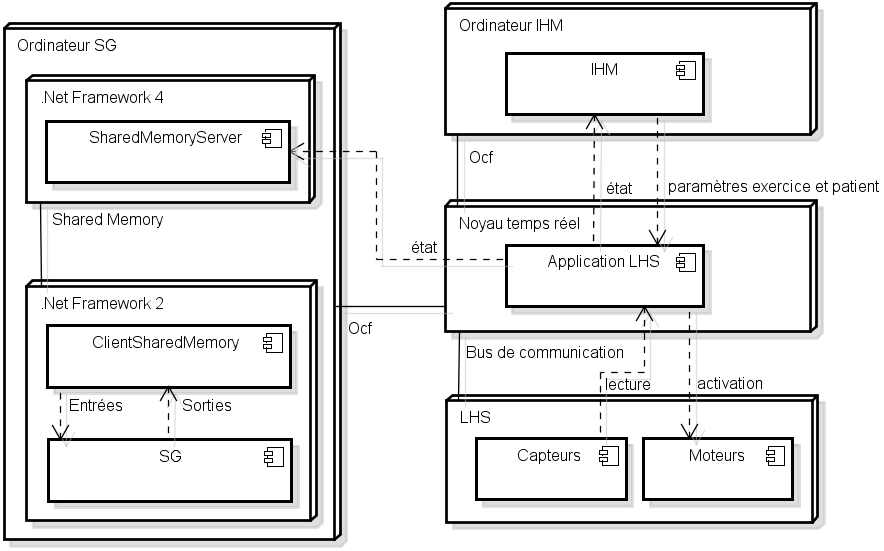
\includegraphics[width=\textwidth]{img/Conception_CommunicationDeploymentDiagram_Resized.png}}
			\captionof{figure}{Diagramme de déploiement montrant les différents composants et leurs interactions.}
			\label{DeploymentClassDiagram}
		\end{minipage}\medskip%TODO: En annexes, voir laisser une miniature ici aussi
				
		Cette structure nécessite donc l'implémentation d'un programme agissant en tant que serveur pour la mémoire partagée, d'une API agissant en tant que client et d'une librairie contenant les classes communes à s'échanger. Un diagramme de classe (présent dans les annexes) montre cette structure ainsi que l'abstraction du contrôleur d'entrées/sorties qui permettra la création d'un simulateur afin de tester le SG sans le LHS.
		
		Afin de garantir le temps réel, le serveur ne se contente pas de récupérer les valeurs quand on le lui demande. Dans un \textit{thread} supplémentaire, il récupère constamment les valeurs présentes dans l'application temps réel et les met à disposition du client. Le client lit ces dernières valeurs et aucune attente n'est effectuée sur une requête réseau. Cette solution, bien qu'elle ne garantisse pas le temps réel de l'interaction, peut utiliser d'anciennes valeurs si les requêtes Ocf ne sont pas terminées \cite{ZanniniRapport}.